\chapter{Kompressionsalgorithmen}

\section{(exakte) LZ77-Kompression}
Der im Folgenden beschriebene Algorithmus für die Generierung einer exakten LZ77-Faktorisierung dient als Referenz für die Evaluation der approximativen Algorithmen.

\subsection{Konzept}
Wie bereits in Kapitel xx beschrieben, erzeugen Algorithmen der LZ77 - Familie eine Faktorisierung einer Eingabezeichenfolge $S$, wobei die Faktoren entweder Referenzen
zu vorherigen Zeichenfolgen oder einzelne Zeichen sein können. Im Rahmen der exakten LZ77 - Faktorisierung wird ein Greedy - Ansatz verwendet, um von links nach rechts 
stets die längste Zeichenfolge zu referenzieren, die bereits links von der aktuellen Position vorkommt.
\begin{algorithm}[ht]
\centering
\caption{COMP$_{LZ77}$} \label{alg:complz77}
\algorithmicrequire $S=e_1...e_n$
\algorithmicensure $F=f_1...f_z$
\begin{algorithmic}
    \STATE $SA \gets SuffixArray(S)$
    \STATE $(NSV, PSV) \gets (NSVArray(S, SA), PSVArray(S, SA))$
    \STATE $F \gets \emptyset$
    \STATE $k \gets 1$
    \WHILE{$k \leq n$}
    \STATE $(len, ref) \gets (0, 0)$
    \STATE $l_{nsv} \gets LCP(S(NSV[k]..n), S(k..n))$
    \STATE $l_{psv} \gets LCP(S(PSV[k]..n), S(k..n))$
    \IF{$l_{nsv} > l_{psv}$}
        \STATE $(len, ref) \gets (l_{nsv}, NSV[k])$
    \ELSIF{$l_{nsv} < l_{psv}$}
        \STATE $(len, ref) \gets (l_{psv}, PSV[k])$
    \ELSE
        \STATE $(len, ref) \gets (0, S[k])$
    \ENDIF
    \STATE $F \gets F + (len, ref)$
    \STATE $k \gets k + len + 1$
    \ENDWHILE
    \RETURN $F$
\end{algorithmic}
\end{algorithm}
In \ref{alg:complz77} wird der Algorithmus zur Generierung einer exakten LZ77-Faktorisierung beschrieben. Der Algorithmus erzeugt zunächst ein SuffixArray, welches allen
Suffixen der Eingabe eine lexikographische Ordnung zuweist. Mithilfe der loxikographischen Ordnung können Kandidaten für Referenzen effizient gefunden werden. Hierfür 
werden mit Hilfe des SuffixArrays zwei Arrays, das Next Smaller Value(NSV) und das Previous Smaller Value(PSV) erzeugt. Sei die aktuelle Position in der Eingabe $k$, so
muss aufgrund von positionellen und lexikographischen Einschränkungen die Position $ref$ der längsten vorherigen Referenz $NSV[k]$ oder $PSV[k]$ sein. Die maximale
Länge der übereinstimmenden Präfixe zwischen $S(NSV[k]..n)$ und $S(k..n)$ bzw. $S(PSV[k]..n)$ und $S(k..n)$ wird durch die Funktion $LCP$ berechnet. Das Ergebnis
dieser Berechnung bestimmt den Faktor $(len, ref)$, welcher in der Eingabe an Position $k$ beginnt. Der Algorithmus terminiert, wenn die gesamte Eingabe abgearbeitet wurde.

\subsection{Theoretisches Laufzeit- und Speicherverhalten}
Die Berechnung des SuffixArrays und die folgende Berechnung der NSV- und PSV-Arrays können mithilfe von Algorithmen aus der Literatur(siehe xx) in $O(n)$ Laufzeit 
durchgeführt werden. In der abschließenden Schleife repräsentiert die $k$-te Iteration den $k$-ten Faktor, wobei die Iteration für die Berechnung der Faktorlänge
$O(|f_k|)$ Laufzeit benötigt. Damit ergibt sich eine Gesamtlaufzeit von $O(n +\underbrace{\sum_{i=1}^{z} |f_i|}_{n}) = O(n)$ für die Generierung der exakten LZ77-Faktorisierung.
Der Speicherbedarf des Algorithmus beträgt $O(n)$, da sich die Größe des SuffixArrays und der NSV- und PSV-Arrays linear zur Eingabelänge verhalten. Es sollte jedoch
angemerkt werden, dass die Linearität des Speicherbedarfs einen hohen konstanten Faktor hat und unabhängig von der Beschaffenheit der Eingabe und der Anzahl der Faktoren ist.

\section{Approximation der LZ77-Faktorisierung(Approx. LZ77)}
\subsection{Konzept}
Im Rahmen dieser Arbeit wird die erste Phase einer speichereffizienten Approximation des LZ77-Algorithmus betrachtet, welche auch eine verlustfreie Kompression darstellt. Wie in
\cite{ApproxLZ77} beschrieben, kann die Kombination aller drei Phasen des Algorithmus eine 2-Approximation bezüglich der Faktorrate ermöglichen. Die resultierenden Faktoren entsprechen
jedoch dem LZ77-Schema, sodass eine verlustfreie Dekompression mit \ref{alg:decomp} möglich ist. Im weiteren Verlauf werden wir die sequenzielle erste Phase des Algorithmus als 
Approx.LZ77 bezeichnen. Im Gegensatz zur exakten LZ77-Faktorisierung werden Referenzen nicht durch einen Greedy-Ansatz mit einem Scan von links nach rechts gefunden. Stattdessen wird 
eine Approximation der exakten LZ77-Faktorisierung erzeugt, die einen Tradeoff zwischen der Faktorrate und der Performanz, hier der Speicherverbrauch, des Algorithmus darstellt. Die
resultierenden Faktoren sind insbesondere dadurch definiert, dass ihre Länge einer Zweierpotenz entspricht. Analog dazu gehen wir ohne Beschränkung der Allgemeinheit davon aus, dass
die Länge der Eingabe ebenfalls eine Zweierpotenz ist. Eine abweichende Eingabelänge kann stets durch entsprechendes Padding erreicht werden. Die Approximation wird in mehreren Runden
durchgeführt, wobei in jeder Runde die noch unverarbeitete Eingabe in Blöcke gleicher Größe eingeteilt wird. Innerhalb einer Runde werden für Zeichenfolgen, die durch die jeweiligen
Blöcke repräsentiert werden, Referenzen, also vorherige Vorokommen, gesucht. Im Erfolgsfall wird ein entsprechender Faktor extrahiert und der Block gilt als markiert. Die verbleibenden
Blöcke werden im Übergang zur nächsten Runde in der Hälfte geteilt. Der Algorithmus terminiert, wenn die Eingabe vollständig verarbeitet wurde, was spätestens nach $log_2(|S|)$ Runden
der Fall ist, da Blöcke der Größe 1 nicht weiter geteilt werden können. Die Zeichenfolgen der Blöcke, die in der letzten Runde nicht markiert wurden, werden als einzelne Zeichen interpretiert
und faktorisiert. Der Ablauf des Algorithmus wird in \ref{alg:compapproxlz77} dargestellt. Initial wird die Eingabe in $2^r$ Blöcke gleicher Größe eingeteilt, wobei $r$ die initiale Runde beschreibt.
Daraufhin wird eine Schleife über alle Runden gestartet, wobei in jeder Iteration die aktuelle Menge der Blöcke auf Referenzen untersucht und ggf. markiert werden. Die Menge der markierten Blöcke,
die auch zur Menge der Faktoren $F$ hinzugefügt werden, wird in der Routine ProcessRound bestimmt. Nachdem die Menge der Blöcke um die markierten Blöcke bereinigt wurde, werden die verbleibenden
Blöcke halbiert und die nächste Runde initiiert.
\begin{algorithm}[ht]
\centering
\caption{COMP$_{ApproxLZ77}$} \label{alg:compapproxlz77}
\algorithmicrequire $S=e_1...e_n$
\algorithmicensure $F=f_1...f_z$
\begin{algorithmic}[1]
    \STATE $F \gets \emptyset$
    \STATE $r \gets 1$
    \STATE $Blocks[1..2^r] \gets InitBlocks(S, 2^r)$ \algorithmiccomment{Split S into $2^r$ equal blocks}
    \WHILE{$r \leq log_2(|S|)$}
        \STATE $markedBlocks[1..z_r] \gets ProcessRound(r, S, Blocks, F)$
        \STATE $Blocks \gets NextNodes(Blocks\setminus markedBlock[1..z_r])$ \algorithmiccomment{Halve unmarked blocks}
        \STATE $r \gets r+1$
    \ENDWHILE
    \RETURN $F$
\end{algorithmic}
\end{algorithm}

Die Funktionsweise der ProcessRound-Routine wird in \ref{alg:processround} beschrieben. Die Ausführung kann in drei Schritte unterteilt werden. Im ersten Schritt werden die Tabellen RFPTable und RefTable
mithilfe der Routine InitTables initialisiert. Die RFPTable ordnet jedem einzigartigen Rabin-Karp-Fingerprint(RFP), der über die Menge aller Blöcke erzeugt wird, den linksten Block zu, welcher diesen 
Wert aufweist. In diesem Rahmen vernachlässigen wird explizit Kollisionfälle des RFP und gehen davon aus, dass die Gleichheit der RFPs zweier Zeichenfolgen ebenfalls die Gleichheit der Zeichenfolgen impliziert.
Die RefTable speichert für jeden Block die Position des linkesten Vorkommens seiner Zeichenfolge in der Eingabe, die zum aktuellen Zeitpunkt bekannt ist.
Die Routine InitTables, wie in \ref{alg:inittables} beschrieben, erzeugt die RFPTable, indem alle Blöcke von links nach rechts durchlaufen werden und das Paar aus einem Block und dessen RFP in die Tabelle
nur dann eingefügt wird, wenn der RFP noch nicht vorhanden ist. Als Konsequenz wird für jeden RFP, der eine einzigartige Zeichenfolge repräsentiert, der entsprechende linkeste Block gespeichert. Die RefTable
wird analog initialisiert. Falls der RFP eines Blocks bereits in der RFPTable vorhanden ist, so kann dem Block ein vorheriges Vorkommen zugeordnet werden. Andernfalls ist der Block das linkeste Vorkommen seiner
Zeichenfolge und dessen Position wird entsprechend gespeichert. Es ist zu betonen, dass die InitTables-Routine durch Aktualisierungen der RefTable bereits markierte Blöcke bzw. Faktoren erzeugt.

Im zweiten Schritt werden zusätzliche Referenzen innerhalb der gesamten Eingabe S gesucht. Dazu wird der RFP eines Fensters der Größe $\frac{|S|}{2^r}$ über die Eingabe berechnet und mit den Einträgen der
RFPTable verglichen. Im Falle eines Treffers wird die Position des Fensters ggf. in der RefTable eingetragen. Im Rahmen des Scans wird ein Rolling-Hash verwendet, um die RFPs der Fenster effizient um eine
Position zu verschieben. 
Schließlich wird im dritten Schritt die RefTable genutzt, um die markierten Blöcke zu bestimmen. Ein Block wird markiert, wenn die Position des linksten Vorkommens seiner Zeichenfolge in der RefTable kleiner
als die aktuelle Position des Blocks ist. Die markierten Blöcke werden in die Menge der Faktoren $F$ eingefügt, wobei die Reihenfolge der Faktoren entweder während des Einfügens oder durch eine nachfolgende
Sortierung sichergestellt werden muss.
\begin{algorithm}[ht]
    \centering
    \caption{ProcessRound} \label{alg:processround}
    \algorithmicrequire $r, S, Blocks$
    \algorithmicensure $markedBlocks$
    \begin{algorithmic}[1]
        \STATE $(RFPTable, RefTable) \gets InitTables(Blocks)$
        \STATE $ReferenceScan(S, Blocks, RFPTable, RefTable)$
        \FOR {$i \gets 1$ \TO $|Blocks|$}
            \IF{$RefTable[i] < Blocks[i].Pos$}
                \STATE $markedBlocks.insert(i)$
                \STATE $F.insert(\frac{|S|}{2^r}, RefTable[i])$ \algorithmiccomment{Ordered Insert}
            \ENDIF
        \ENDFOR
        \RETURN $markedBlocks$
    \end{algorithmic}
    \end{algorithm}

\begin{algorithm}[ht]
\centering
\caption{InitTables} \label{alg:inittables}
\algorithmicrequire $Blocks$
\algorithmicensure $RFPTable, RefTable$
\begin{algorithmic}[1]
    \STATE $RFPTable \gets HashTable[RFP, LeftMostBlock]$
    \STATE $RefTable[1..|S|] \gets (0,...,0)$
    \FOR{$i \gets 1$ \TO $|Blocks|$}
        \STATE $RFP \gets RFP(Blocks[i])$
        \IF{$RFP \textbf{ in } RFPTable$}
            \STATE $RefTable[i] \gets RFPTable[RFP].Pos$
        \ELSE
            \STATE $RFPTable.insert(RFP,Blocks[i])$
            \STATE $RefTable[i] \gets Blocks[i].Pos$
        \ENDIF
    \ENDFOR
    \RETURN $RFPTable, RefTable$
\end{algorithmic}
\end{algorithm}

\begin{algorithm}[ht]
\centering
\caption{ReferenceScan} \label{alg:refscan}
\algorithmicrequire $S, Blocks, RFPTable, RefTable$
\begin{algorithmic}
    \STATE blockSize $\gets \frac{|S|}{|Blocks|}$
    \STATE $RFP \gets RFP(S[1..blockSize])$
    \FOR{$i \gets 1$ \TO $|S|-blockSize$}
        \IF{$RFP in RFPTable$ \AND $i < RefTable[RFPTable[RFP]]$}
            \STATE $RefTable[RFPTable[RFP]] \gets i$
        \ENDIF
        \STATE $RFP \gets RFP(S[i+1..i+blockSize])$ \algorithmiccomment{Rolling Hash}
    \ENDFOR
\end{algorithmic}
\end{algorithm}


\subsection{Theoretisches Laufzeit- und Speicherverhalten}
Die Laufzeit des Algorithmus wird durch die Anzahl der Runden und der Extraktion von Referenzen in jeder Runde bestimmt. Die Anzahl der Runden beträgt maximal $log_2(|S|)=log_2(n)$. In jeder Runde
werden Referenzen innerhalb der Blöcke durchd die InitTables-Routine bestimmt. Die Menge aller Blöcke, die in dieser Routine bearbeitet werden, decken maximal die gesamte Eingabe S ab. Die Laufzeit
der Routine erhält durch die Berechnung des RFPs über dieser Zeichenfolge eine Laufzeitschätzung von $O(n)$. Die Referenzsuche über die gesamte Eingabe durch die ReferenceScan-Routine benötigt ebenfalls
$O(n)$ Laufzeit, da des berücksichtigte Fenster in linearer Zeit über die Eingabe verschoben werden kann. Die Laufzeit der ProcessRound-Routine beträgt somit $O(n)$. Insgesamt ergibt sich eine
Gesamtlaufzeit von $O(n \cdot log_2(n))$ für die Generierung der approximativen LZ77-Faktorisierung. Der Speicherbedarf des Algorithmus wird durch die Größe der RFPTable und der RefTable bestimmt, die
wiederum durch die Anzahl der Blöcke bestimmt wird. In jeder Runde repräsentiert die Menge der Blöcke die noch unverarbeitete Eingabe, sodass aus jedem Block im Laufe des Algorithmus mindestens ein
Faktor extrahiert wird. Die Anzahl der Blöcke in der Runde übersteigt damit nie die Anzahl der endgültigen Faktoren. Der Speicherbedarf kann damit konservativ auf $O(z)$ abgeschätzt werden.

\section{Parallelisierung von Approx. LZ77(Approx. LZ77Par)}
\subsection{Konzept}
Im Folgenden beschreiben wir das verwendete Schema zur Parallelisierung des Approx. LZ77-Algorithmus. Die Parallelisierung zielt auf eine schrittweise Bearbeitung der Eingabe, die jeweils
auf die verschiedenen Prozessoren bzw. Threads verteilt werden. 
\begin{figure}[h]
    \centering
    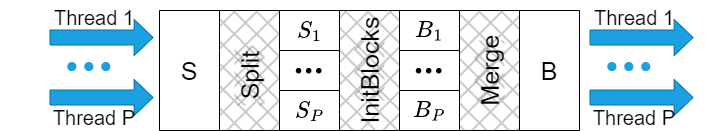
\includegraphics[width=0.8\textwidth]{Images/parallel_initnodes.png}
    \caption{Parallele Generierung der initialen Blöcke}
    \label{fig:parinitnodes}
\end{figure}
In \ref{fig:parinitnodes} wird die parallele Generierung der initialen Blöcke dargestellt. Hiebrei wird die Eingabe $S$ in $P$ Teile aufgebrochen, sodass die Routine InitBlocks auf jedem Prozessor
die zugehörigen Blöcke erzeugen kann. Da die chronologische Ordnung erhalten bleibt, können die erzeugten Blöcke ohne zusätzlichen Aufwand kombiniert werden.

\begin{figure}[h]
    \centering
    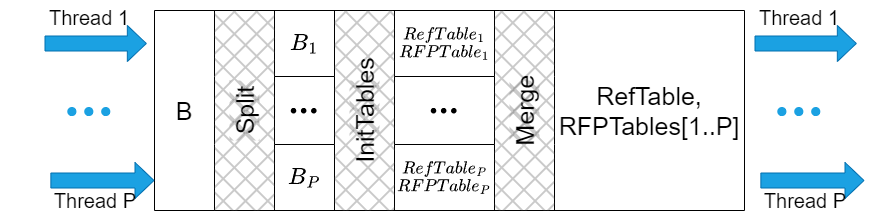
\includegraphics[width=0.8\textwidth]{Images/parallel_inittables.png}
    \caption{Parallele Initialisierung der RFP-Tabelle und der Referenztabelle}
    \label{fig:parinittables}
\end{figure}
In \ref{fig:parinittables} wird die parallele Initialisierung der RFP-Tabelle und der Referenztabelle dargestellt. Die Menge aller Blöcke wird in $P$ Teile aufgeteilt, wobei als Kriterium für die
Aufteilung der RFP jedes Blocks verwendet wird. Als Konsequenz werden identische Zeichenfolgen nicht auf verschiedene Prozessoren verteilt. Jeder Prozessor erzeugt eine eigene RFP-Tabelle, wobei
die Referenztabelle durch alle Prozessoren gemeinsam aktualisiert wird. Auch hier wird durch den Aufteilungsschlüssel eine Überlappung der Zugriffe vermieden. Das Ergebnis ist eine konsistente
Referenztabelle und eine eine Menge von P RFP-Tabellen, die jeweils eine klar definierte Teilmenge der RFPs enthalten.

\begin{figure}[h]
    \centering
    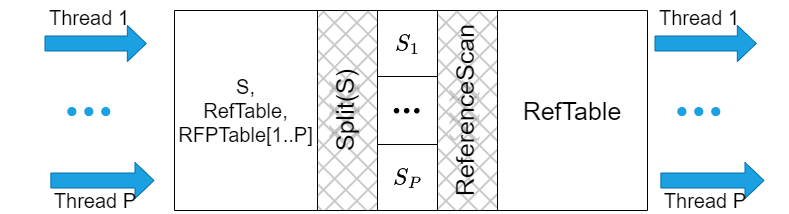
\includegraphics[width=0.8\textwidth]{Images/parallel_referencescan.png}
    \caption{Paralleler Scan der Eingabe nach zusätzlichen Referenzen}
    \label{fig:parrefscan}
\end{figure}
In \ref{fig:parrefscan} wird der parallele Scan der Eingabe S nach zusätzlichen Referenzen dargestellt. Die Eingabe S wird in $P$ Teile aufgeteilt. Auf jede Teilmenge wird die sequenzielle Routine
ReferenceScan angewendet, wobei die Referentabelle durch alle Prozessoren gemeinsam aktualisiert wird und ein paralleler Lesezugriff auf die RFP-Tabellen stattfindet. 

Schließlich müssen die implizit erzeugten Faktoren in die Menge der Faktoren $F$ eingefügt werden. Da die Reihenfolge der Faktoren erhalten bleiben muss, wird eine nachträgliche parallele Sortierung
verwendet. Die Implementierung der parallelen Sortierung ist jedoch nicht Gegenstand dieser Arbeit und wird daher nicht weiter betrachtet. Eine mögliche Implementierung ist in [] beschrieben.

\subsection{Theoretisches Laufzeit- und Speicherverhalten}
Eine theoretische Laufzeit von $O(\frac{n \log n}{p})$ kann erreicht werden, wobei $p$ die Anzahl der Prozessoren ist. Der Speicherbedarf des Algorithmus beträgt $O(z)$. Dies stellt jedoch eine
ideale Abschätzung dar, die in der Praxis nicht erreicht werden kann. Insbesondere die Interaktion mit dem Speicher und die Kommunikation zwischen den Prozessoren führen zu einer oberen Schranke
des Speedups.

\section{Praktische Optimierungen}
Im Folgenden betrachten wir optionale Optimierungen, die die durchschnittliche Laufzeit von Approx. LZ77 verbessern können auf Kosten von anderen Metriken. Jede einzelne Technik ist unabhängig von
den anderen nutzbar, wobei eine positive Korrelation zu erwarten ist.

\subsection{Dynamische Endrunde(DynEnd) - Laufzeit vs. Qualität*}
Sei eine Kodierung $K$ für die Übersetzung der erzeugten Faktorenfolge $F$ gegeben. Der Wert,
\begin{equation}
    Min^{Ref}_{Bin}=min\{|K(f)| | f \in F ,f \text{ ist Referenz}\}
\end{equation}
gibt die minimale Anzahl an Bits an, die für die Kodierung einer Referenz benötigt wird. Analog dazu beschreibt
\begin{equation}
    Max^{Lit}_{Bin}=max\{|K(f)| | f \in F, f \text{ ist Zeichen}\}
\end{equation}
die maximale Anzahl an Bits, die für die Kodierung eines einzelnen Zeichens benötigt wird. Sei $f_{ref}$ ein beliebiger referenzierender Faktor, welcher 
$|f_{ref}|\leq\frac{Min^{Ref}_{Bin}}{Max^{Lit}_{Bin}}$ Zeichen referenziert. Die referenzierte Zeichenfolge von $f_{ref}$ wird im Folgenden als $S_{ref}$ mit $|S_{ref}|=|f_{ref}|$ bezeichnet.
Dann gilt für die Länge der kodierten Repräsentation von $f_{ref}$:
\begin{equation}
\begin{split}
    |K(f_{ref})| & \geq Min^{Ref}_{Bin}\\
    & \geq |f_{ref}| \cdot Max^{Lit}_{Bin}\\
    & \geq \sum_{i=1}^{|f_{ref}|} |K((0, S_{ref}(i)))|.
\end{split}
\end{equation}
Es folgt, dass ein referenzierender Faktor, dessen Länge eine obere Schranke von $\frac{Min^{Ref}_{Bin}}{Max^{Lit}_{Bin}}$ Zeichen nicht überschreitet, nicht effizient kodiert werden kann.
Stattdessen sollten die referenzierten Zeichen einzeln kodiert werden. Die Technik der dynamischen Endrunde greift diese Idee auf, indem Referenzen unterhalb einer Grenzlänge nicht berechnet
werden. Gibt uns die Kodierung eine Grenzlänge $l^{ref}_{min}$ vor, so kann der Algorithmus in Runde $r = \lceil log_2{|S|}-log_2{l^{ref}_{min}} \rceil$ terminieren. Da potenziell 
referenzierende Faktoren aufgebrochen werden, kann die Qualität der Faktorisierung sinken, wobei das binäre Endprodukt kleiner wird. Es ergibt sich also eine steigende Faktorrate bei
sinkender Kompressionsrate.
\begin{equation}
    CR^{Approx.LZ77}_{DynEnd} \leq CR^{Approx.LZ77}
\end{equation}
\begin{equation}
    FR^{Approx.LZ77}_{DynEnd} \geq FR^{Approx.LZ77}
\end{equation}

\subsection{Dynamische Startrunde(DynStart) - Laufzeit vs. Speicher} \label{sec:dynstart}
Gegeben seien zwei initiale Runden $r_{init1}$ und $r_{init2}$ mit $1\leq r_{init1} < r_{init2}\leq log_2{|S|}$, die auf der gesamten Eingabe S angewendet werden, 
so wird die Eingabe jeweils in $2^{r_{init1}}$ bzw. $2^{r_{init2}}$ Blöcke gleicher Größe eingeteilt. Die Menge der Blöcke werde im Folgenden als $B_{init1}$ bzw. $B_{init2}$ bezeichnet.
Im Rahmen der Bearbeitung der Runden wird eine Menge von markierten Blöcken $B_{init1}^{marked}\subset B_{init1}$ bzw. $B_{init2}^{marked}\subset B_{init2}$ erzeugt, für die ein vorheriges
Vorkommen bestimmt wurde. Aufgrund der Natur der Blockhalbierung in jeder Runde, kann jedem Block in $B_{init1}$ eine Gruppe von $2^{r_{init2}-r_{init1}}$ Blöcken in $B_{init2}$ zugeordnet
werden, die die gleiche Zeichenfolge repräsentieren. Die Folgerung lässt sich insbesonere auch auf die markierten Blöcke anwenden, sodass die folgende Beziehung hergeleitet werden kann:
\begin{equation}
    |B^{init2}_{marked}| \geq 2^{r_{init2}-r_{init1}} \cdot |B^{init1}_{marked}|.
\end{equation}
Weiterhin folgt, dass die Existenz eines markierten Blocks in $B^{init1}$ die Existenz von $2^{r_{init2}-r_{init1}}$ benachbarten markierten Blöcken in $B^{init2}$ impliziert. Die
Umkehrung dieser Aussage liefert,
\begin{equation}
    longestChain(B^{init2}_{marked}) < 2^{r_{init2}-r_{init1}} \Rightarrow B^{init1}_{marked}=\emptyset, 
\end{equation}
wobei $LongestChain(B^{init2}_{marked})$ die längste Kette von benachbarten markierten Blöcken in $B^{init2}_{marked}$ bezeichnet.
Die Technik der dynamischen Startrunde greift diese Beziehung auf, indem initial die Runde $r_{init}=log_2{|S|}/2$ auf die gesamte Eingabe S angewendet wird. Im Anschluss
kann der Wert $longestChain(B^{init}_{marked})$ mithilfe eines Scans über die markierten Blöcke bestimmt werden. Der errechnete Wert impliziert eine Runde $r_{Start}$ derart,
dass vorherige Runden garantiert keine markierten Blöcke erzeugen und damit ausgelassen werden können. Der Wert $r_{Start}$ ergibt sich wie folgt,
\begin{equation}
    r_{Start} = r_{init}-
    \begin{cases}
        -1, & \text{falls } longestChain(B^{init}_{marked}) = 0\\
        \lfloor log_2{longestChain(B^{init}_{marked})} \rfloor, & \text{sonst}
    \end{cases}
\end{equation}
In Abhängigkeit von der Beschaffenheiit der Eingabe, können maximal die Hälfte aller Runden ausgelassen werden, ohne eine Veränderung der Ergebnisse zu verursachen. In
Runde $r_{init}=log_2{|S|}/2$ werden jedoch $2^{log_2{|S|}/2}=\sqrt{|S|}$ Blöcke erzeugt. Dies führt zu einer weiteren unteren Schranke für den Speicheraufwand des Algorithmus.
Falls diese Technik angewandt wird, kann der Speicheraufwand mit $O(\max\{\sqrt{n}, z\})$ abgeschätzt werden.

\subsection{Vorberechnete Runde(PreMatching) - Laufzeit vs. Speicher}
Analog zu der dynamischen Startrunde kann eine vorberechnete Runde ebenfalls genutzt werden, um den Arbeitsaufwand vorheriger Runden zu reduzieren. Sei $r_{prematch} mit 
1\leq r_{prematch} \leq log_2{|S|}$ eine Runde, die auf die gesamte Eingabe angewendet wird. Als Ergebnis erhalten wir die Menge der markierten Blöcke $B_{prematch}^{marked}$.
Weiterhin speichern wir uns den RFP aller Blöcke, die im Rahmen der Runde erzeugt werden. Wie in \ref{sec:dynstart} gezeigt, kann jedem Block in einer vorherigen Runde einer Gruppe
von Blöcken in einer späteren Runde zugeordnet werden, die die gleiche Zeichenfolge repräsentieren. Die Konkatenation von Zeichenfolgen kann entsprechend \ref{eq:concat} in eine
konstante Operation auf der Basis des RFP übersetzt werden. Gegeben sei eine Runde $r_m$ mit $1\leq r_m \leq log_2{|S|}$. Für einen beliebigen Block $b \in B_m$ können $2^{r_{prematch}-r_m}$
viele Böcke $(b_1, b_2, ..., b_{2^{r_{prematch}-r_m}})\in B_{prematch}$ gefunden werden, die die gleiche Zeichenfolge repräsentieren. So ergibt sich für den zugehörigen RFP,
\begin{equation}
    RFP(b) = RFP(b_1) \oplus RFP(b_2) \oplus ... \oplus RFP(b_{2^{r_{prematch}-r_m}})
\end{equation}
, wobei jede Operation in konstanter Zeit durchgeführt werden kann. Die Anzahl der Rechenschritte für die Berechnung des RFP eines Blockes hängt nun nicht mehr von der Länge der
repräsentierten Zeichenfolge ab, sondern Rundendistanz zur vorberechneten Runde.
Weiterhin kann die Menge der unmarkierten Blöcke $B_{prematch}^{unmarked}=B_{prematch}\setminus B_{prematch}^{marked}$ genutzt werden, um die Menge der Blöcke $B_m$ in Runde $r_m$
zu reduzieren. Ein Block $b \in B_m$ kann nur dann markiert werden, wenn die equivalente Sequenz von Blocken $(b_1, b_2, ..., b_{2^{r_{prematch}-r_m}})\in B_{prematch}$ markiert ist.
Die Umkehrung dieser Aussage liefert einen Filter für alle vorherigen Runden. Die zusätzlich gespeicherten Daten erhöhen den Speicherbedarf des Algorithmus. Falls die vorberechnete
Runde auf den Wert $k\in \mathbb{N}$ festgelegt wird, so kann der Speicherbedarf mit $O(\max\{2^k, z\})$ abgeschätzt werden.

\subsection{Minimale Tabellengröße(ScanSkip) - Laufzeit vs. Qualität}
Wie in \ref{alg:inittables} beschrieben, wird die RFP-Tabelle und die Referenztabelle durch die InitTables-Routine initialisiert. Im Rahmen der Routine werden alle Blöcke auf Duplikate
überprüft, sodass nur einzigartige Blöcke in die RFP-Tabelle eingefügt werden und die Referenztabelle implizite Faktoren speichert. Die Anzahl der Blöcke, die im folgenden Schritt 
in der Referencescan-Routine\ref{alg:refscan} markeirt werden können, ist durch die Anzahl der Einträge in der RFP-Tabelle beschränkt. Der Wert $k\in [0,1]$ gebe den Anteil der
Einträge in der RFP-Tabelle in Relation zur Anzahl der Blöcke an. Unsere Optimierung sieht vor, dass in jeder Runde die Referencescan-Routine nur angewendet wird, falls $k$ größer
als ein Schwellwert $k_{min}\in [0,1]$ ist. Faktoren, die durch die ausgelassene Suche in dieser Runde nicht erzeugt wurden, werden in einer der nächsten Runden ausgegeben, wobei diese
durch die Halbierung der Blöcke sukzessive in ihrer Anzahl verdoppelt werden. Damit sinkt zwangsläufig die Faktorrate, wobei die ausgelassen Referenzsuche einen zeitlichen Gewinn bringt.
Es wurde bereits etabliert, dass die Anzahl der Blöcke in jeder Runde durch die Anzahl der Faktoren, z, beschränkt ist. Damit ist die Anzahl der Faktoren, die durch diese Technik nicht
direkt ausgegeben werden, stets kleiner als $k_{min} \cdot z$ und weiterhin bei der Ausgabe durch $2 \cdot k_{min} \cdot z$ beschränkt. In der Gesamtheit aller Runden ergibt sich dadurch
auf einer obere Schranke für die relative Verschlechterung der Faktorrate um den Faktor $k_{min} * 2^{log_2{|S|}}$, wobei diese Schätzung sehr konservativ ist.